\documentclass[letter, 12pt]{article}

\usepackage{amsmath,amsthm,amssymb}
\usepackage{fancyhdr}
\usepackage{geometry}
\usepackage{enumerate}
\usepackage{enumitem}
\usepackage{listings}
\usepackage{algorithm}
\usepackage{hyperref}
\usepackage{algorithmic}
\usepackage{eqparbox}
\usepackage{float}
\usepackage{bm}
\usepackage{bbm}
\usepackage{mathtools}
\usepackage{minted}
\usepackage{forest}
\usepackage{cite}

\author{Shengjie Li}
\title{CS 536 : Computing Solutions}

\pagestyle{fancy}
\fancyhf{} 
\lhead{Shengjie Li \\ netID: sl1560}
\cfoot{\thepage} 
\renewcommand{\headrulewidth}{1pt}
\renewcommand{\headwidth}{\textwidth}
\renewcommand\algorithmiccomment[1]{%
    \hfill\#\ \eqparbox{COMMENT}{#1}%
}
\newlist{subquestion}{enumerate}{1}
\setlist[subquestion, 1]{label = \alph*)}
\DeclareMathOperator*{\argmax}{arg\,max}
\DeclareMathOperator*{\argmin}{arg\,min}

\setlength\parindent{0pt}

% margin adjustment
\addtolength{\textwidth}{1in}
\addtolength{\oddsidemargin}{-0.5in}
\addtolength{\evensidemargin}{-0.5in}
\addtolength{\topmargin}{-.5in}
\addtolength{\textheight}{1.0in}
\setlength\parindent{0cm}

\begin{document}
    \centerline{\textbf{CS 536 : Computing Solutions}}
    \section{Linear Regression}
    \begin{enumerate}
    	\item {}
    	\par{As fig. \ref{fig:q1-1} and \ref{fig:q1-2} shows, the weights and bias of the model I got were pretty close to the true weights and bias. But there was still some noise in the weights of my model.}
    	\par{My model concluded $ x_1 $ as the most significant feature, and $ x_{11} $ as the least significant feature. Due to the insufficient of the data, my model concluded $ x_{11} $ as the least significant feature. When the size of data set becomes 100,000, the weights of my model are shown in fig. \ref{fig:q1-3}, which are indeed pretty close to the true weights.}
    	\par{When $ m = 100,000 $, the `true' error I got was 0.10375875.}
    	\begin{figure}[H]
    		\centering
    		\begin{minipage}{.48\textwidth}
    			\centering
    			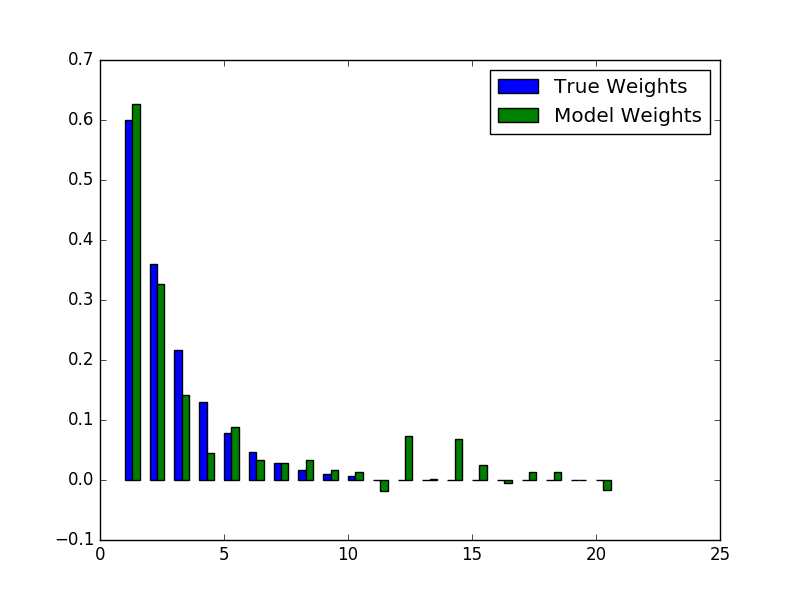
\includegraphics[width=\linewidth]{q1-1.png}
    			\caption{Comparison of true weights and the weights of model.}
    			\label{fig:q1-1}
    		\end{minipage}
	    	\begin{minipage}{.48\textwidth}
		    	\centering
		    	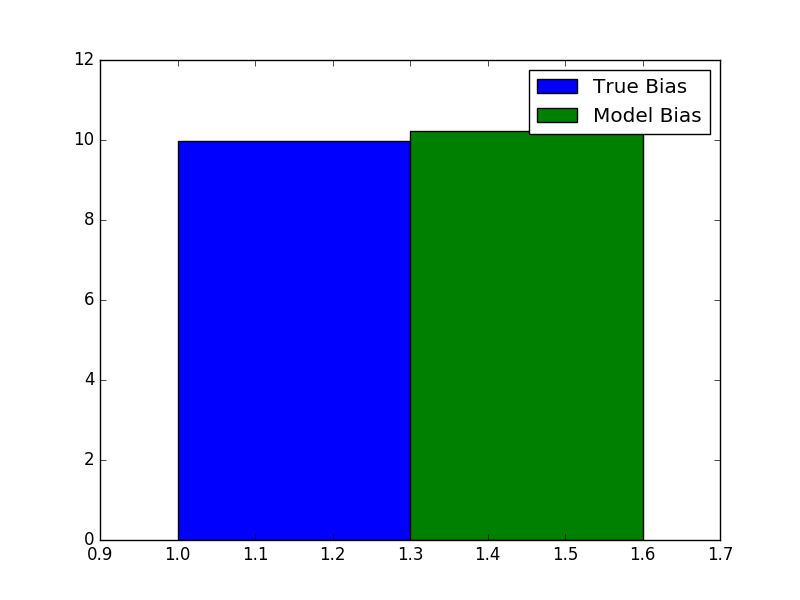
\includegraphics[width=\linewidth]{q1-2.png}
		    	\caption{Comparison of true bias and the bias of model.}
		    	\label{fig:q1-2}
		    \end{minipage}
    	\end{figure}
	    \begin{figure}[H]
		    \centering
		    \centering
		    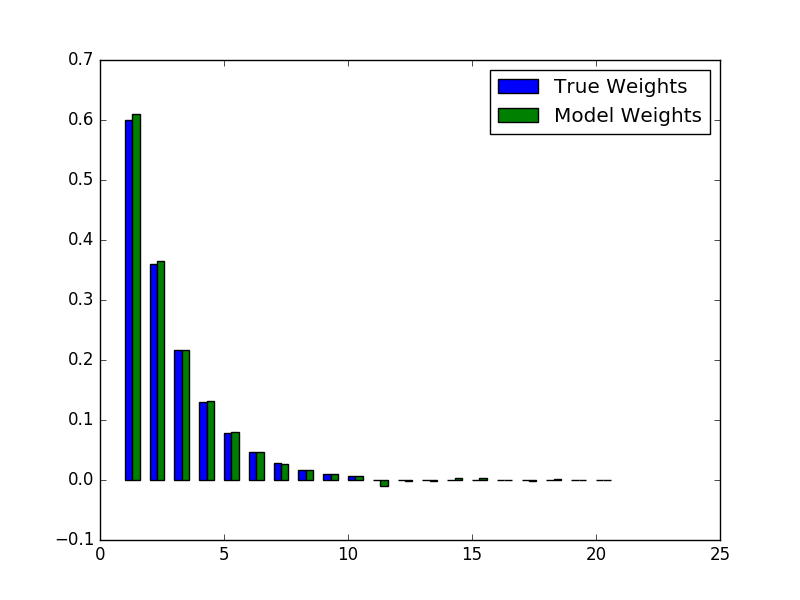
\includegraphics[width=0.7\linewidth]{q1-3.png}
		    \caption{The weights of model when m = 100,000.}
		    \label{fig:q1-3}
		\end{figure}
    	
    	\item {}
    	\par{As fig. \ref{fig:q2-1} shows, the optimal $ \lambda $ is 0.05, which yields an optimal error of 0.10415862.}
    	\par{As fig. \ref{fig:q2-2} and \ref{fig:q2-3} shows, the bias of the model I got was pretty close to the true bias. But the weights were not really ideal, because it should have pruned some features. There's still some space for improvement.}
    	\par{My model concluded $ x_1 $ as the most significant feature, and $ x_{11} $ as the least significant feature. Due to the insufficient of the data, my model concluded $ x_{11} $ as the least significant feature. When the size of data set becomes 100,000, the weights of my model are shown in fig. \ref{fig:q2-4}, which are indeed pretty close to the true weights.}
    	\par{When $ m = 1000 $, the model I got using ridge regression was somehow similar to that of naive linear regression, but have smaller weights.}
    	\begin{figure}[H]
    		\centering
    		\centering
    		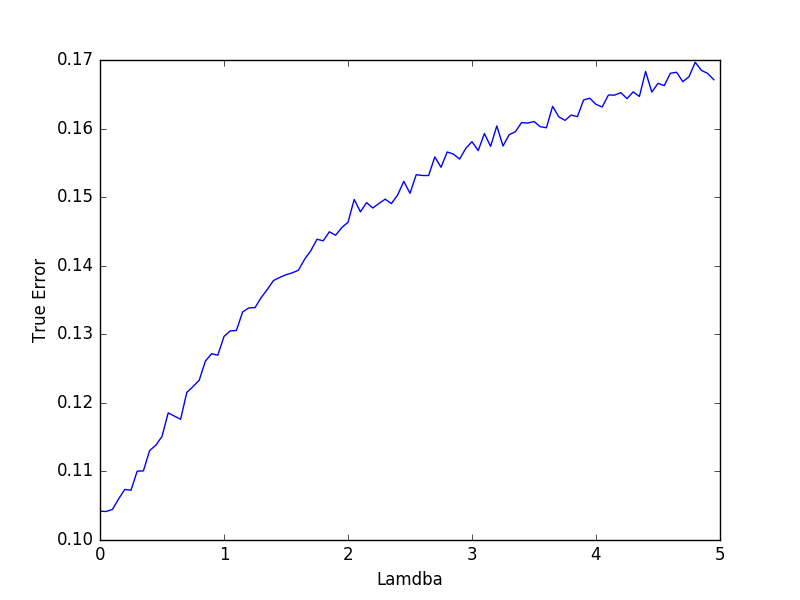
\includegraphics[width=0.7\linewidth]{q2-1.png}
    		\caption{True errors vs lambdas.}
    		\label{fig:q2-1}
    	\end{figure}
    	\begin{figure}[H]
    		\centering
    		\begin{minipage}{.48\textwidth}
    			\centering
    			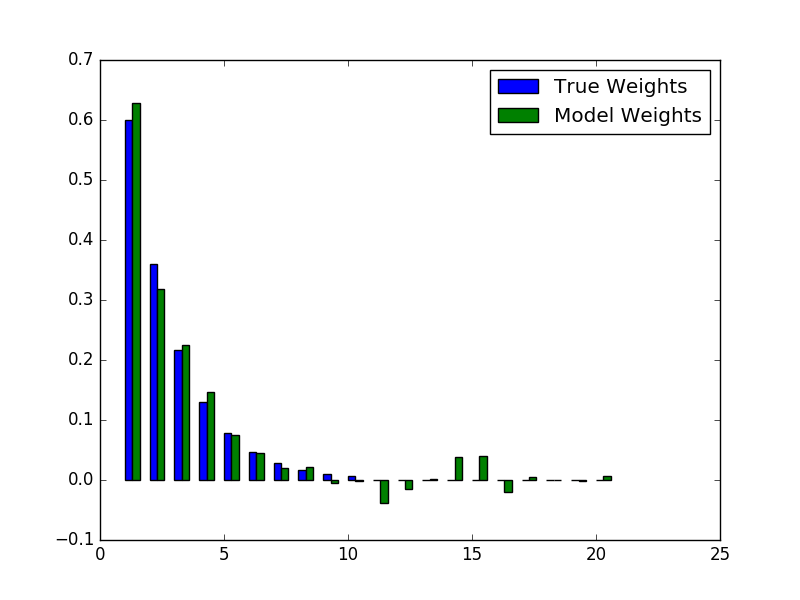
\includegraphics[width=\linewidth]{q2-2.png}
    			\caption{Comparison of true weights and the weights of model.}
    			\label{fig:q2-2}
    		\end{minipage}
    		\begin{minipage}{.48\textwidth}
    			\centering
    			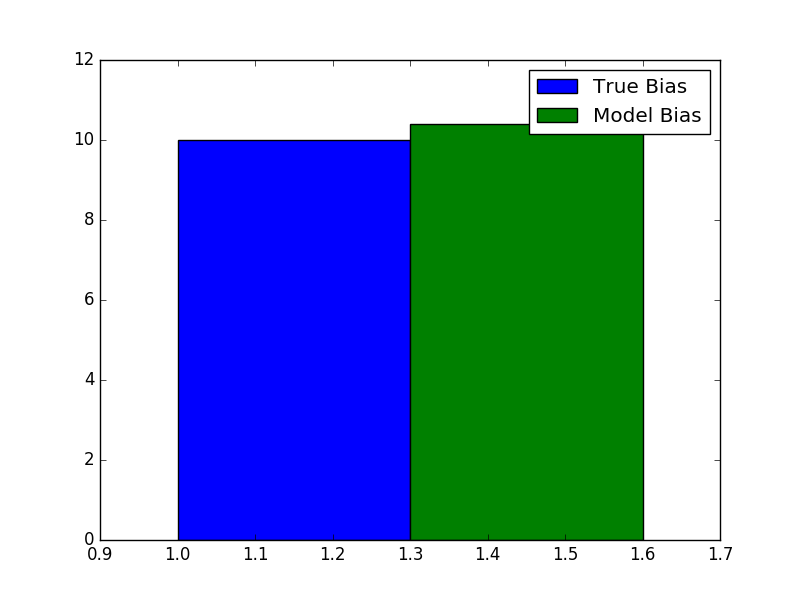
\includegraphics[width=\linewidth]{q2-3.png}
    			\caption{Comparison of true bias and the bias of model.}
    			\label{fig:q2-3}
    		\end{minipage}
    	\end{figure}
	    \begin{figure}[H]
		    \centering
		    \centering
		    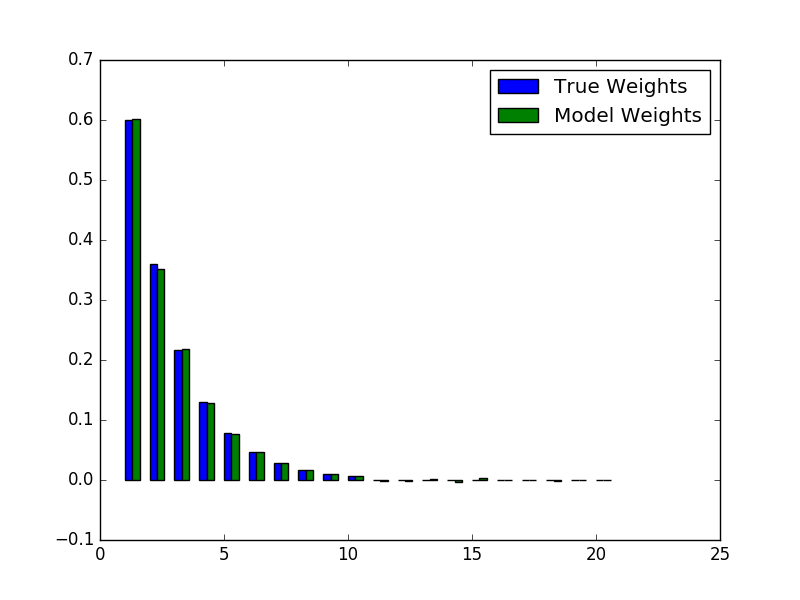
\includegraphics[width=0.7\linewidth]{q2-4.png}
		    \caption{The weights of model when m = 100,000.}
		    \label{fig:q2-4}
		\end{figure}
    	
    	\item {}
    	\par{As fig. \ref{fig:q3-1} shows, as $ \lambda $ increases, the number of zero-weighted features increases.}
    	\begin{figure}[H]
    		\centering
    		\centering
    		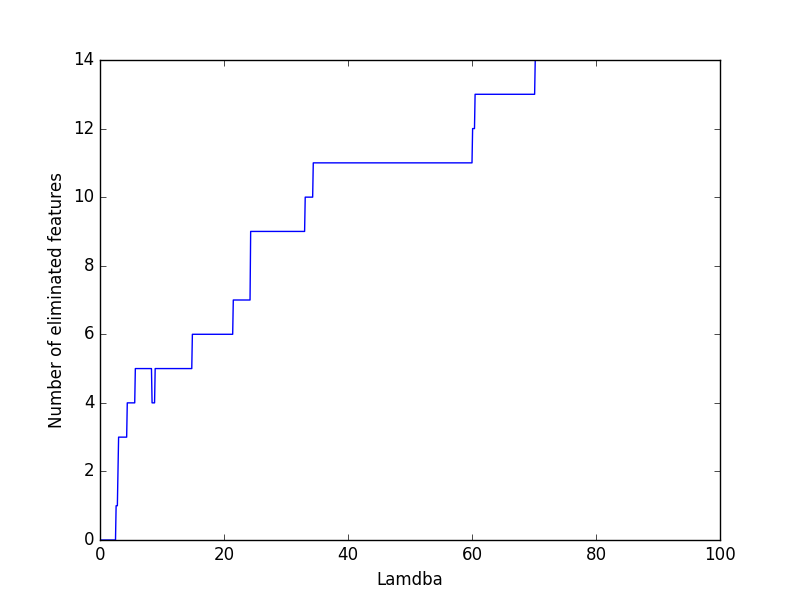
\includegraphics[width=0.7\linewidth]{q3-1.png}
    		\caption{Number of eliminated features vs lambda when m = 1000.}
    		\label{fig:q3-1}
    	\end{figure}
    
    	\item {}
    	\par{As fig. \ref{fig:q4-1} shows, the optimal $ \lambda $ is 17.4, which yields an optimal error of 0.09864528.}
    	\par{As fig. \ref{fig:q4-2} and \ref{fig:q4-3} shows, the bias of the model I got was pretty close to the true bias. Most of the weights were close to the true weights, especially weights for those unrelated features. But there are still some strange behaviors for $ x_4, x_5, x_{11}, x_{12}, x_{13} $.}
    	\par{My model concluded $ x_1 $ as the most significant feature, and $ x_{11} $ as the least significant feature. Due to the insufficient of the data, my model concluded $ x_{11} $ as the least significant feature. When the size of data set becomes 100,000, the weights of my model are shown in fig. \ref{fig:q2-4}, which are indeed pretty close to the true weights.}
    	\par{When $ m = 1000 $, the model I got using ridge regression was somehow similar to that of naive linear regression, but have smaller weights.}
    	\begin{figure}[H]
    		\centering
    		\centering
    		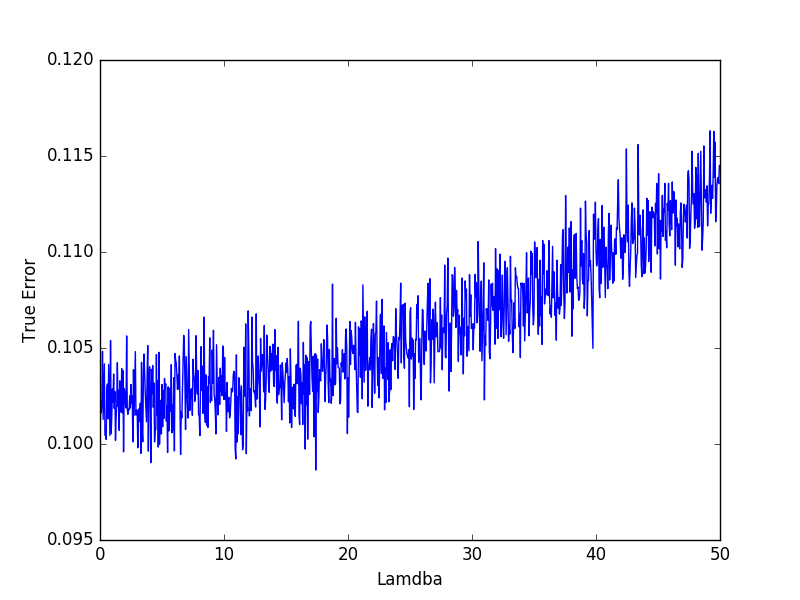
\includegraphics[width=0.7\linewidth]{q4-1.png}
    		\caption{True errors vs lambdas.}
    		\label{fig:q4-1}
    	\end{figure}
    	\begin{figure}[H]
    		\centering
    		\begin{minipage}{.48\textwidth}
    			\centering
    			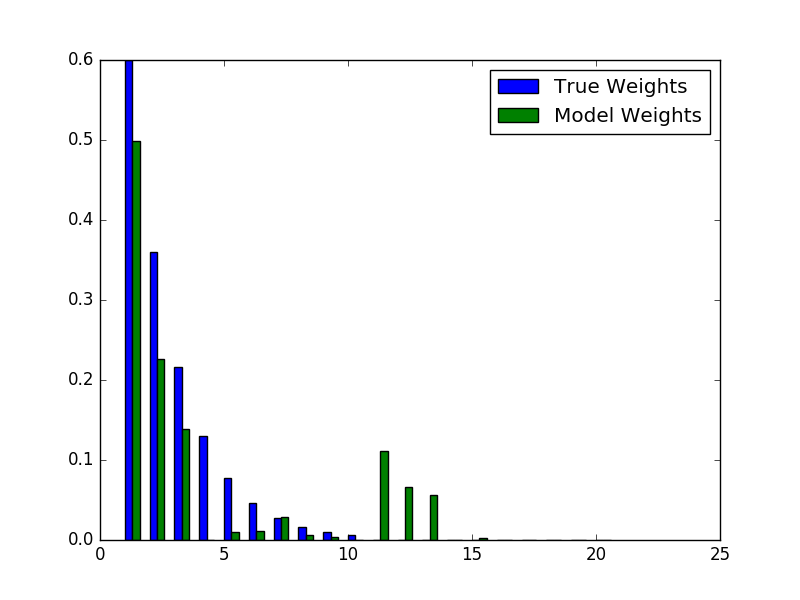
\includegraphics[width=\linewidth]{q4-2.png}
    			\caption{Comparison of true weights and the weights of model.}
    			\label{fig:q4-2}
    		\end{minipage}
    		\begin{minipage}{.48\textwidth}
    			\centering
    			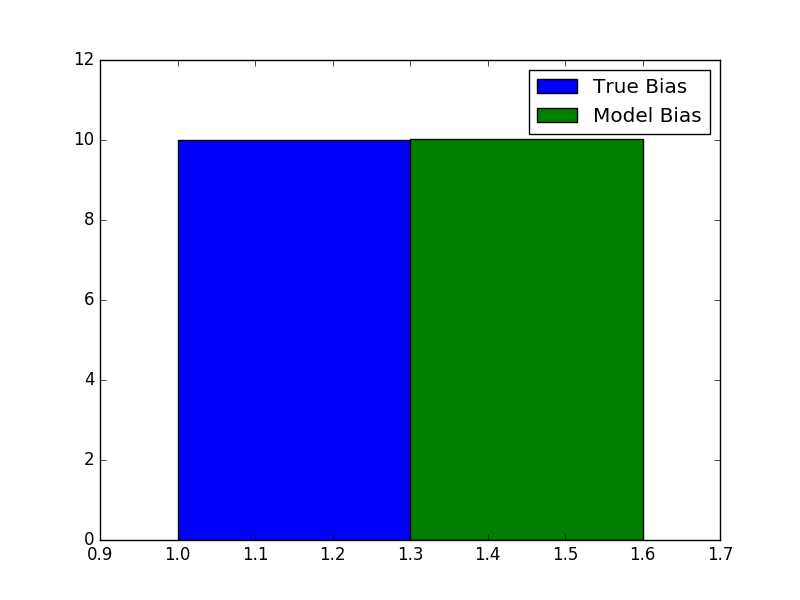
\includegraphics[width=\linewidth]{q4-3.png}
    			\caption{Comparison of true bias and the bias of model.}
    			\label{fig:q4-3}
    		\end{minipage}
    	\end{figure}
    	\item {}
    \end{enumerate}
    \section{SVMs}
\end{document}
